\documentclass[a4paper]{article}

%% Language and font encodings
\usepackage[english]{babel}
\usepackage[utf8x]{inputenc}
\usepackage[T1]{fontenc}
\usepackage[section]{placeins}
\usepackage{graphicx}
\usepackage{caption}
\usepackage{subcaption}

\usepackage{fancyvrb}	

%\usepackage{pdfpages}%to insert pdfs
 
\usepackage{float}		%Ben trying to format figures

%% Sets page size and margins
\usepackage[a4paper,top=3cm,bottom=2cm,left=3cm,right=3cm,marginparwidth=1.75cm]{geometry}

%% Useful packages
\usepackage{amsmath}
\usepackage{graphicx}
\usepackage[colorinlistoftodos]{todonotes}
\usepackage[colorlinks=true, allcolors=blue]{hyperref}
\makeatletter

%% All below Added by Ben |||||||||||||||||||||||||||||||||||||||||||||||
\g@addto@macro\@floatboxreset\centering
\makeatother				% this and above automatically center figures

% Alphabetized list macro from:  https://tex.stackexchange.com/questions/121489/alphabetically-display-the-items-in-itemize
\usepackage{datatool}% http://ctan.org/pkg/datatool
\newcommand{\sortitem}[1]{%
  \DTLnewrow{list}% Create a new entry
  \DTLnewdbentry{list}{description}{#1}% Add entry as description
}
\newenvironment{sortedlist}{%
  \DTLifdbexists{list}{\DTLcleardb{list}}{\DTLnewdb{list}}% Create new/discard old list
}{%
  \DTLsort{description}{list}% Sort list
  \begin{itemize}%
    \DTLforeach*{list}{\theDesc=description}{%
      \item \theDesc}% Print each item
  \end{itemize}%
}
%use these instead to alphabetize list:
%\begin{sortedlist}
%   \sortitem{ISDYNSTP
%
%||||||||||||||||||||||||||||||||||||||||||||||||||||||||||||||||||||||||||


\title{ECE271, Final Project}
\author{Ben Adams, Grant Haines, Benjiman Walsh}
\date{\today}

\begin{document}
\maketitle

\pagebreak

\tableofcontents

\section{Introduction}

The purpose of this project is to create a digital logic design that uses various input modules with various output modules.



\section{High Level Descriptions}%%%%%%%%%%%%%%


\section{Controller Descriptions}

This section is meant to provide a brief but thorough low-level view of the operations of our chosen input devices. 

\subsection{NES Controller}

The Nintendo Entertainment System (NES) first became available in America in 1985 and revolutionized society as the first accessible home video game system. NES controllers work by receiving "clock" and "latch" signals from the NES console and transmitting a data signal to the console. NES controllers use a shift register to store all of the controller's button data when the console sends the latch signal (As in figure \ref{nesSchematic}). Each successive clock signal shifts the controller register down and the controller's data wire outputs a value that represents the next button's signal (See figure \ref{nesClock}). 


\begin{figure}[H]
    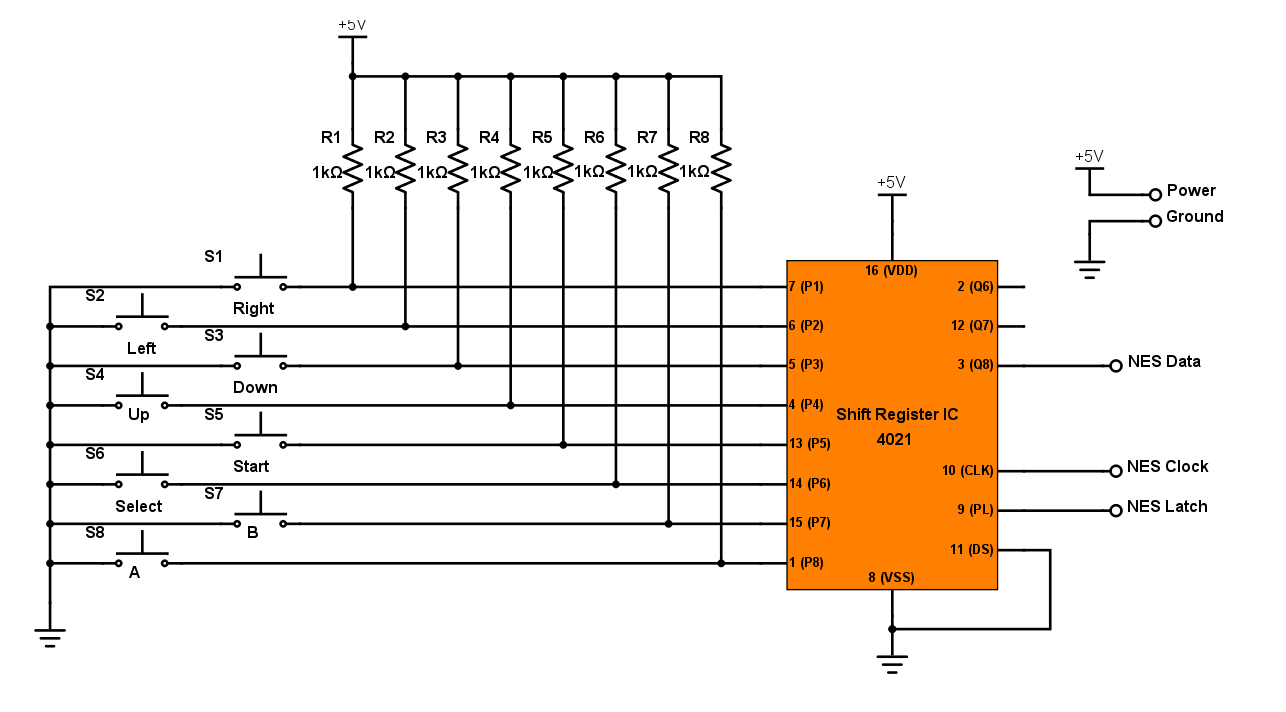
\includegraphics[width=0.8 \linewidth]{images/nesSchema.png}
    \caption{"Button Mashing" on the NES}
    \label{nesSchematic}
\end{figure}


\begin{figure}[H]
    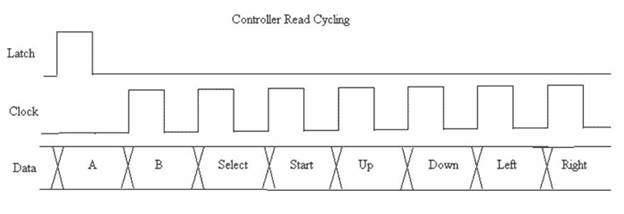
\includegraphics[width=0.8 \linewidth]{images/nesclock.jpg}
    \caption{"Button Mashing" on the NES}
    \label{nesClock}
\end{figure}

The NES controller decoder SystemVerilog module was provided for us in the course materials.

\section{HDL Components}



\section{Appendix}

\subsection{Source Code}%%%%%%%%%%%%%%%%%%%%%%%%%%%%%%%%%%%

\subsubsection{NES Controller Reader}



\subsubsection{Square Wave Generator}

\begin{Verbatim}[tabsize=4]
module periodTime(input logic clk,
					input logic [2:0] data,
					output logic q);
					
int compareNumber;
int count;

always_comb
		case(data)
			0: compareNumber = 6400;	// just mod input clock until audio spectrum periods
			1: compareNumber = 3200;	// one octave
			2: compareNumber = 1600;
			3: compareNumber = 8000;
			
			4: compareNumber = 4000;
			5: compareNumber = 2000;
			6: compareNumber = 1000;
			7: compareNumber = 500;		// consider adding default case
		endcase
			
always_ff @(posedge clk)
	begin
		if (count >= compareNumber)	// could modify to not restart notes when changed
			count <= 0;
		else 
			count <= count +1;
	end

always_comb
	begin
			if( count < compareNumber)				
				q = (count > compareNumber/2); 	//assigns output with initial low
			else 
				q = 0;
	end

endmodule
\end{Verbatim}

\subsubsection{VGA Output}

\begin{Verbatim}
module vgaOutput
		(input clock50MHz,
		 input inReset,
		 input inRed,
		 input inGreen,
		 input inBlue,
		 output hSync,
		 output vSync,
		 output [3:0] outRed, outGreen, outBlue);
	
	vga_counter #(.N(4)) redCounter (
		.clk(inRed),
		.reset(inReset),
		.q(redCount)
	);
	
	vga_counter #(.N(4)) greenCounter (
		.clk(inGreen),
		.reset(inReset),
		.q(greenCount)
	);
	
	vga_counter #(.N(4)) blueCounter (
		.clk(inBlue),
		.reset(inReset),
		.q(blueCount)
	);

	clockDivBy2 clockDivider(
		.clock50MHz(clock50MHz),
		.inReset(~inReset),
		.outClock(clock25MHz)
	);
	
	vga_hCounterComp #(.a(10'd96), .b(10'd48), .c(10'd640), .d(10'd16)) hSyncCounter (
		.inClock(clock25MHz),
		.clock50MHz(clock50MHz),
		.inReset(~inReset),
		.signal(hSync),
		.displaySignal(hSignal)
	);
	
	clockDivBy2 syncDivider(
		.clock50MHz(hSync),
		.inReset(~inReset),
		.outClock(hClock)
	); 
	
	vga_vCounterComp #(.a(10'd2), .b(10'd33), .c(10'd480), .d(10'd10)) vSyncCounter (
		.inClock(hClock),
		.clock50MHz(clock50MHz),
		.inReset(~inReset),
		.signal(vSync),
		.displaySignal(vSignal)
	);
	
	vga_displayMux display (
		.select(hSignal & vSignal),
		.inRed(redCount),
		.inGreen(greenCount),
		.inBlue(blueCount),
		.outRed(outRed),
		.outGreen(outGreen),
		.outBlue(outBlue)
	);

endmodule
\end{Verbatim}

\subsection{Simulation Results}%%%%%%%%%%%%%%%%%%%%%%%%%%%%%

\subsubsection{NES Controller Reader}
\begin{figure}[H]
    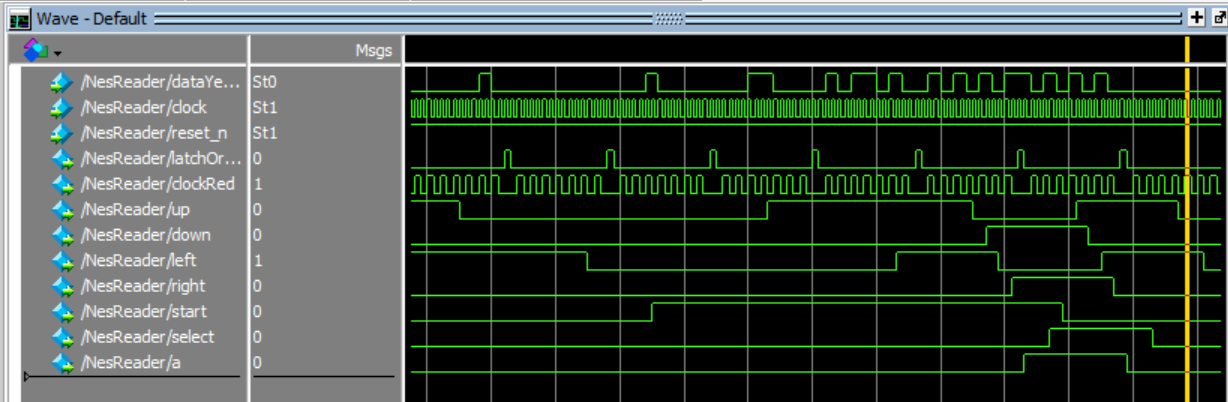
\includegraphics[width=0.8 \linewidth]{images/NESSIM.png}
    \caption{"Button Mashing" on the NES}
    \label{nesButtonMash}
\end{figure}

At first, I wanted to test the NES controller reader by just simulating a bunch of random inputs as seen in Figure \ref{nesButtonMash}. I remembered the NES game CONTRA had a cheat code that involved most of the controller's buttons (all but SELECT). The "Contra Code" was then simulated I'm gonna rewrite this.
 
\begin{figure}[H]
    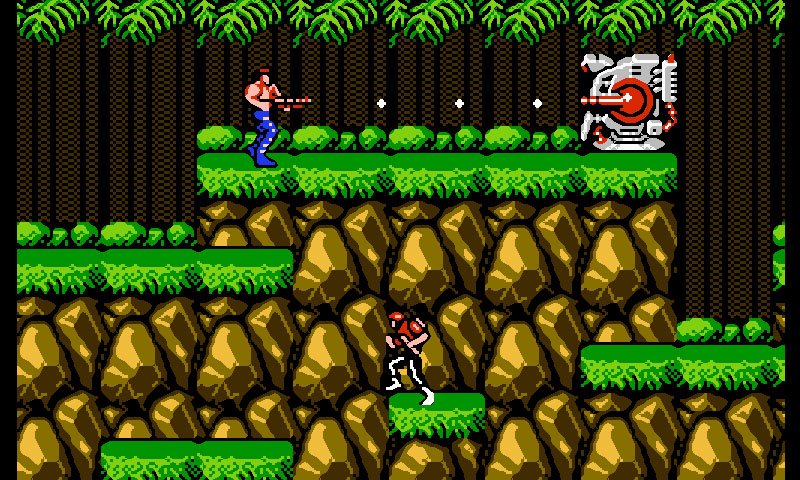
\includegraphics[width=0.8 \linewidth]{images/contra.jpg}
    \caption{CONTRA screenshot}
    \label{contra}
\end{figure}

\begin{figure}[H]
    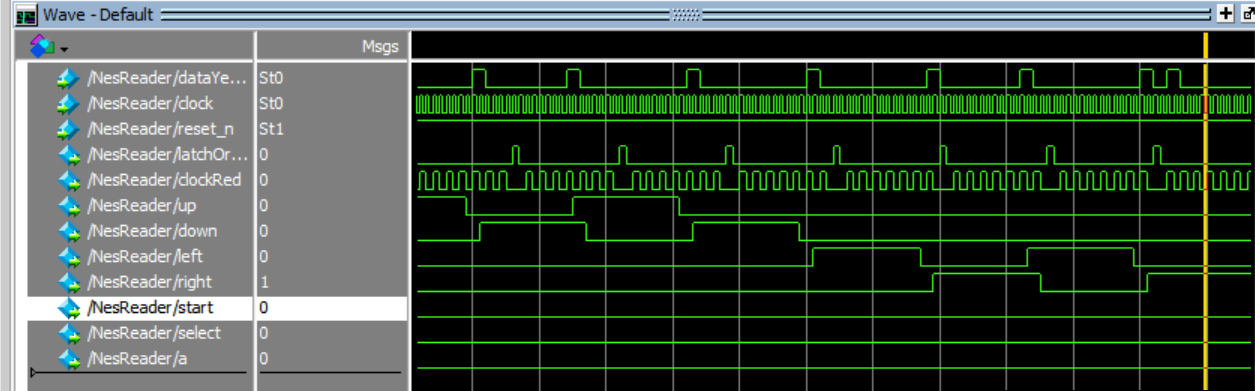
\includegraphics[width=0.8 \linewidth]{images/NESSIMcontra.png}
    \caption{Simulating the "Contra Code" }
    \label{contraSim}
\end{figure}

\begin{verbatim}

force -freeze sim:/NesReader/dataYellow 0 0, 0 {20 ps} , 0 {40 ps} , 0 {60 ps} , 
    1 {80 ps} , 0 {100 ps} , 0 {120 ps} , 0 {140 ps}	#up
force -freeze sim:/NesReader/dataYellow 0 0, 0 {20 ps} , 0 {40 ps} , 0 {60 ps} , 
    0 {80 ps} , 1 {100 ps} , 0 {120 ps} , 0 {140 ps}	#down
force -freeze sim:/NesReader/dataYellow 0 0, 0 {20 ps} , 0 {40 ps} , 0 {60 ps} , 
    1 {80 ps} , 0 {100 ps} , 0 {120 ps} , 0 {140 ps}	#up
force -freeze sim:/NesReader/dataYellow 0 0, 0 {20 ps} , 0 {40 ps} , 0 {60 ps} , 
    0 {80 ps} , 1 {100 ps} , 0 {120 ps} , 0 {140 ps}	#down
force -freeze sim:/NesReader/dataYellow 0 0, 0 {20 ps} , 0 {40 ps} , 0 {60 ps} , 
    0 {80 ps} , 0 {100 ps} , 1 {120 ps} , 0 {140 ps}	#left
force -freeze sim:/NesReader/dataYellow 0 0, 0 {20 ps} , 0 {40 ps} , 0 {60 ps} , 
    0 {80 ps} , 0 {100 ps} , 0 {120 ps} , 1 {140 ps}	#right
force -freeze sim:/NesReader/dataYellow 0 0, 0 {20 ps} , 0 {40 ps} , 0 {60 ps} , 
    0 {80 ps} , 0 {100 ps} , 1 {120 ps} , 0 {140 ps}	#left
force -freeze sim:/NesReader/dataYellow 0 0, 0 {20 ps} , 0 {40 ps} , 0 {60 ps} , 
    0 {80 ps} , 0 {100 ps} , 0 {120 ps} , 1 {140 ps}	#right
force -freeze sim:/NesReader/dataYellow 0 0, 1 {20 ps} , 0 {40 ps} , 0 {60 ps} , 
    0 {80 ps} , 0 {100 ps} , 0 {120 ps} , 0 {140 ps}	#b	
force -freeze sim:/NesReader/dataYellow 1 0, 0 {20 ps} , 0 {40 ps} , 0 {60 ps} , 
    0 {80 ps} , 0 {100 ps} , 0 {120 ps} , 0 {140 ps}	#a
force -freeze sim:/NesReader/dataYellow 0 0, 0 {20 ps} , 0 {40 ps} , 1 {60 ps} , 
    0 {80 ps} , 0 {100 ps} , 0 {120 ps} , 0 {140 ps}	start
\end{verbatim}

\subsubsection{Square Wave Generator}

\begin{figure}[H]
    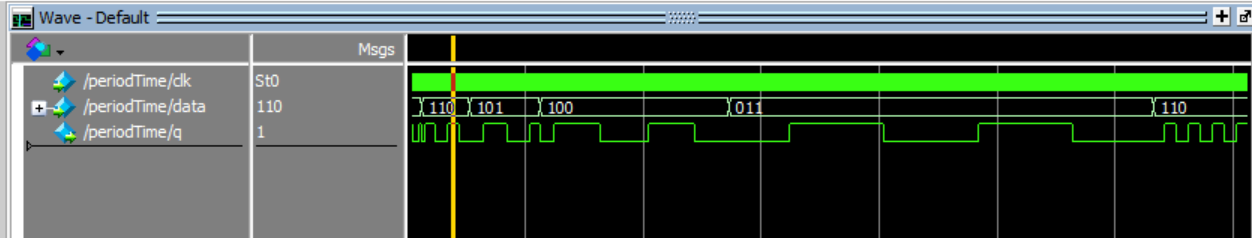
\includegraphics[width=0.8 \linewidth]{images/squareSim.png}
    \caption{Simulating button inputs to control the square wave oscillator}
    \label{squareSim}
\end{figure}


%\includepdf[page=-]{Ch3Example}

\end{document}
